%!TEX root = ../Thesis.tex

%%%%%%%%%%%%%%%%%%%%%%%%%%%%%%%%%%%%%%%%%%%%%%%%%%%%%%%%%%%%%%%%%%%%%%%%
\chapter{Results}
\label{chap:Results}

The result of this thesis is a novel edge bundling algorithm that uses a Physarium Steiner tree calculation to build a structure that can then use to bundle the paths. As mentioned in \autoref{sec:testing}, we generated the graphs that we then compared to the Edge-Path bundling approach by Wallinger et al. \cite{wallinger_edge-path_2022}, and the Winding Roads method by Lambert et al. \cite{lambert_winding_2010}, as these have made their algorithms readily available, we already have a good understanding of how they work, and they are representative of a method with an underlying structure and one without one.

%%%%%%%%%%%%%%%%%%%%%%%%%%%%%%%%%%%%%%%%%%%%%%%%%%%%%%%%%%%%%%%%%%%%%%%%

\section{Quality Metrics}
%%%%%%%%%%%%%%%%%%%%%%%%%%%%%%%%%%%%%%%%%%%%%%%%%%%%%%%%%%%%%%%%%%%%%%%%

\begin{figure}[t]
    \centering
    \begin{subfigure}{0.3\linewidth}
        \centering
        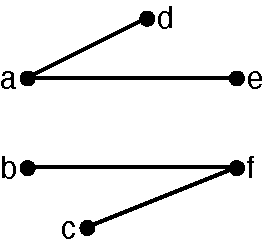
\includegraphics[width=0.9\linewidth]{figures/amb_value/0_amb_value.pdf}
        \caption{Straight-line graph}
        \label{fig:amb_value_0}
    \end{subfigure}
    \begin{subfigure}{0.3\linewidth}
        \centering
        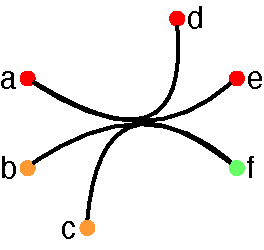
\includegraphics[width=0.9\linewidth]{figures/amb_value/1_amb_value.pdf}
        \caption{Bundled graph}
        \label{fig:amb_value_1}
    \end{subfigure}
  \caption{\subref{fig:amb_value_1} is a possible bundle of \subref{fig:amb_value_0}. In \subref{fig:amb_value_1}, all red nodes are false neighbors $N_{\Gamma}^f$ for the b node, and all yellow nodes are false neighbors $N_{\Gamma}^f$ for f. \cite{Straub2022}}
  \label{fig:ambiguity_2}
\end{figure}

To compare those three algorithms, we utilize the three quality metrics provided by Wallinger et al. \cite{wallinger_edge-path_2022} and modify them according to our needs. 
The ink reduction $ink(I)$ reveals how many edges were bundled and how much the bundling reduced the clutter by counting the non-white pixels in a plot. $I_B$ is the bundled plot and $I_O$ the original plot.

\begin{equation}
    ink(I)=\frac{\sum_{i=1}^m \sum_{j=1}^n I_B(i,j)}{\sum_{i=1}^m \sum_{j=1}^n I_O(i,j)}
\end{equation}

The bundling reduced clutter inside the graph if the number of non-white pixels shrank.
The next metric, $dist(\Gamma)$, tells if the bundled edges make a long detour or remain close to the Euclidean distance. Suppose they had a long detour that would make adjacencies harder to read. 

\begin{equation}
    dist(\Gamma)= \sum_{(u,v)\in E} \frac{d_{\Gamma}(u,v)}{||u-v||}
\end{equation}

The distortion value is calculated by dividing the length of the sum of the edges of the bundled graph by that of the original.
The ambiguity metric $amb(\Gamma)$ reveals the perceivable false connections within the bundled graph.

\begin{equation}
    amb(\Gamma)=\frac{\sum_{v \in V} \sum_{e=(v,w)\in E} |N_{\Gamma}^f(v,e)|}{\sum_{v \in V} \sum_{e=(v,w)\in E} |N_{\Gamma}(v,e)|}
\end{equation}

To calculate this, we divide all false neighbors by all possible neighbors. $N_{\Gamma}$ is the number of reachable neighbors from a node $x$ with edge $e$. $N_{\Gamma}^f$ are all false neighbours. \autoref{fig:ambiguity_2} is an example of the relationship between true and false neighbors.
A connection is ambiguous if two edges intersect with a slight angle or the distance between them is too small to distinguish them.
%%%%%%%%%%%%%%%%%%%%%%%%%%%%%%%%%%%%%%%%%%%%%%%%%%%%%%%%%%%%%%%%%%%%%%%%
% ************************************************************************
\begin{table*}[tb]
  \centering
  \setlength\tabcolsep{5pt} % adjust white space inside table
  \caption{
    \label{tab:quality}
    The table displays the quality metrics scores for our four synthetic data graphs. The bundled drawings for the \textbf{default} graph are displayed here \autoref{fig:default_bezier_steiner}, for the \textbf{10x10} graph here \autoref{fig:10x10_figure}, for the \textbf{15x15} graph here \autoref{fig:15x15_figure} and the \textbf{25x25} graph here \autoref{fig:25x25_figure}.
  }  
  \begin{tabular}{p{0.045\linewidth} || p{0.045\linewidth} p{0.045\linewidth} p{0.055\linewidth} | p{0.045\linewidth} p{0.045\linewidth} p{0.055\linewidth} | p{0.045\linewidth} p{0.045\linewidth} p{0.055\linewidth} | p{0.045\linewidth} p{0.045\linewidth} p{0.055\linewidth}}
    \toprule
     & \multicolumn{3}{c|}{\bfseries default} & \multicolumn{3}{c|}{\bfseries 10x10\_10n\_30e} & \multicolumn{3}{c|}{\bfseries 15x15\_10n\_40e} & \multicolumn{3}{c}{\bfseries 25x25\_10n\_30e}\\
     & $ink$ & $dist$ & $amb$ & $ink$ & $dist$ & $amb$ & $ink$ & $dist$ & $amb$ & $ink$ & $dist$ & $amb$ \\
    \midrule
    Org & 1.000 & 1.000 & 0.000 & 1.000 & 1.000 & 0.035 & 1.000 & 1.00 & 0.037 & 1.00 & 1.00 & 0.100 \\
    WR & 0.686 & \textbf{0.985} & \textbf{0.000} & 0.677 & \textbf{1.055} & 0.070 & 0.700 & \textbf{1.017} & \textbf{0.062} & \textbf{0.643} & \textbf{1.001} & \textbf{0.033} \\
    EPB & 1.553 & 1.321 & \textbf{0.000} & 1.368 & 1.169 & \textbf{0.053} & 1.167 & 1.179 & 0.075 & 1.513 & 1.177 & 0.100 \\
    PSB & \textbf{0.685} & 0.955 & \textbf{0.000} & \textbf{0.613} & 1.060 & 0.122 & \textbf{0.562} & 1.126 & 0.075 & 0.728 & 1.191 & 0.133 \\
    \bottomrule
  \end{tabular}
\end{table*}
% ************************************************************************

\begin{figure}[H]
    \begin{subfigure}{0.5\linewidth}
        \centering
        \includegraphics[width=\linewidth]{figures/10x10/original_10x10_10n_30e.png}
        \caption{Straight-line graph}
        \label{fig:original_10x10}
    \end{subfigure}
    \begin{subfigure}{0.5\linewidth}
        \centering
        \includegraphics[width=\linewidth]{figures/10x10/wr_10x10_10n_30e.png}
        \caption{Winding Roads}
        \label{fig:wr_10x10}
    \end{subfigure}
    \begin{subfigure}{0.5\linewidth}
        \centering
        \includegraphics[width=\linewidth]{figures/10x10/epb_10x10_10n_30e.png}
        \caption{Edge-Path bundling}
        \label{fig:epb_10x10}
    \end{subfigure}
    \begin{subfigure}{0.5\linewidth}
        \centering
        \includegraphics[width=\linewidth]{figures/10x10/10x10_10n_30e_12-1000.png}
        \caption{Physarium Steiner bundling}
        \label{fig:10x10}
    \end{subfigure}
  \caption{These are example solutions for a 10x10 grid graph. The original straight-line graph is presented in \subref{fig:original_10x10}. With these plots, the strike bundling of our method in \subref{fig:10x10} can be seen.
  As all three algorithms use different techniques to plot the graph, slight visual variations may be noticeable.}
  \label{fig:10x10_figure}
\end{figure}

\begin{figure}[H]
    \begin{subfigure}{0.5\linewidth}
        \centering
        \includegraphics[width=\linewidth]{figures/15x15/original_15x15_10n_40e.png}
        \caption{Straight-line graph}
        \label{fig:original_15x15}
    \end{subfigure}
    \begin{subfigure}{0.5\linewidth}
        \centering
        \includegraphics[width=\linewidth]{figures/15x15/wr_15x15_10n_40e.png}
        \caption{Winding Roads}
        \label{fig:wr_15x15}
    \end{subfigure}
    \begin{subfigure}{0.5\linewidth}
        \centering
        \includegraphics[width=\linewidth]{figures/15x15/epb_15x15_10n_40e.png}
        \caption{Edge-Path bundling}
        \label{fig:epb_15x15}
    \end{subfigure}
    \begin{subfigure}{0.5\linewidth}
        \centering
        \includegraphics[width=\linewidth]{figures/15x15/15x15_10n_40e_12-1000.png}
        \caption{Physarium Steiner bundling}
        \label{fig:15x15}
    \end{subfigure}
  \caption{These are example solutions for a 15x15 grid graph. The original straight-line graph is presented in \subref{fig:original_15x15}. Interestingly to us is that \subref{fig:epb_15x15} and \subref{fig:15x15} look similar in regards to their ink reduction, but their metrics in \autoref{tab:quality} do not confirm this observation. This is the only plot out of the three examples where the Physarium Steiner bundling looks similar to one of the other approaches in this chase Edge-Path bundling.
  As all three algorithms use different techniques to plot the graph, slight visual variations may be noticeable.}
  \label{fig:15x15_figure}
\end{figure}

\begin{figure}[H]
    \begin{subfigure}{0.5\linewidth}
        \centering
        \includegraphics[width=\linewidth]{figures/25x25/original_25x25_10n_30e.png}
        \caption{Straight-line graph}
        \label{fig:original_25x25}
    \end{subfigure}
    \begin{subfigure}{0.5\linewidth}
        \centering
        \includegraphics[width=\linewidth]{figures/25x25/wr_25x25_10n_30e_graph.png}
        \caption{Winding Roads}
        \label{fig:wr_25x25}
    \end{subfigure}
    \begin{subfigure}{0.5\linewidth}
        \centering
        \includegraphics[width=\linewidth]{figures/25x25/epb_25x25_10n_30e_graph.png}
        \caption{Edge-Path bundling}
        \label{fig:epb_25x25}
    \end{subfigure}
    \begin{subfigure}{0.5\linewidth}
        \centering
        \includegraphics[width=\linewidth]{figures/25x25/25x25_10n_30e_12-1000.png}
        \caption{Physarium Steiner bundling}
        \label{fig:25x25}
    \end{subfigure}
  \caption{These are example solutions for a 25x25 grid graph. The original straight-line graph is presented in \subref{fig:original_25x25}. With these plots, it is easy to spot the striker bundling approach of \subref{fig:25x25}. All long edges that remain relatively straight and original are merged into the main bundle in the middle.
  As all three algorithms use different techniques to plot the graph, slight visual variations may be noticeable.}
  \label{fig:25x25_figure}
\end{figure}

\section{Comparison}
\label{sec:comparison}

As mentioned in \autoref{sec:testing}, our algorithm is too slow to solve real-world graphs, and we, therefore, rely on synthetic data we generated. The default dataset has six nodes and was the graph we tested new features throughout the testing phase, as it is fast to calculate, and the resulting Steiner tree is known. It is also the only graph that is not randomly generated. The others get increasingly complex and grow in size. The increasing complexity was done to test the limits and see the behavior of the calculation \autoref{tab:quality}. 

\subsection{Ink Reduction}
\label{sec:ink_reduction}
Logically the ink reduction of the straight-line graph is one. Edge path bundling performs the worst in this category as it uses the shortest edges of the existing path network and a B\'{e}zier curve to visualize the longest paths. Winding Roads and our approach have a much higher degree of bundling, as both use an underlying structure to bundle. That the Physarium Steiner bundling comes out on top is to be expected, as it has a smaller frame to work with. The scores also fit the appearance of \autoref{fig:10x10}, \autoref{fig:15x15} and \autoref{fig:25x25}.

\subsection{Distortion}
\label{sec:distortion}
The distortion on a straight-line graph is, by definition, one. With this metric, the results are much closer, and Winding roads has the least distorted bundling. We observe that the distortion value of our approach is linked to the graph size; the larger the graph, the higher the distortion value. The high distortion value means that the greater the graph gets, the longer the detours of the paths must be, compared to their original counterparts. The longer detours exist because all paths must use the Steiner tree for their routing and if the graph increases in size, the detour through the Steiner tree becomes more significant than the direct path.

\subsection{Ambiguity}
\label{sec:ambiguity}
As even straight-line graphs can have ambiguities, it is to be expected that a low ambiguity value is present. Both Winding Roads and Edge Path bundling have only a slightly larger ambiguity value than the straight-line graph. These are caused by edge crossings which a shallow crossing angle. On the other hand, our approach consistently has the most ambiguities as the proximity of paths causes them. This results in a compact graph whose side effect is that it is more challenging to follow paths.
%%%%%%%%%%%%%%%%%%%%%%%%%%%%%%%%%%%%%%%%%%%%%%%%%%%%%%%%%%%%%%%%%%%%%%%%

